%Created by Ali Heydari
%\title{Title page with logo}

\documentclass[12pt]{article}
\usepackage[english]{babel}
\usepackage[utf8x]{inputenc}
\usepackage{amsmath}
\usepackage{graphicx}
\graphicspath{{./images/}}
\usepackage{hyperref}
\usepackage{float}
\usepackage[colorinlistoftodos]{todonotes}





\begin{document}

\begin{titlepage}

\newcommand{\HRule}{\rule{\linewidth}{0.5mm}} 

\center


\includegraphics[scale=0.3]{IUST_logo_color}\\[1cm]
\textsc{\Large Iran University of Science and Technology}\\[1.5cm]
\textsc{Logical Circuit }\\[0.5cm]
%\textsc{\large Minor Heading}\\[0.5cm]



\HRule \\[0.4cm]
{ \huge \bfseries designing washing machine timer circuit}\\[0.4cm]
\HRule \\[1.5cm]

\Large \emph{Author:}\\
Ali \textsc{Heydari}\\[3cm]

{\large \today}\\[2cm]

\vfill

\end{titlepage}


%\begin{abstract}
%abstract
%\end{abstract}

\section{Introduction}

A washing machine is a machine that washes dirty clothes. It contains a barrel into which the clothes are placed. This barrel is filled with water, and then rotated very quickly to make the water remove dirt from the clothes. Most washing machines are made so that detergent (liquids or powders) can be put into the machine.\footnote{\href{https://simple.wikipedia.org/wiki/Washing_machine}{From Wikipedia, the free encyclopedia}} These can help make the clothes cleaner.
\\ In this proposal i decided to design circuite of washing machine timer.

\section{Circuit features}
\label{sec:Circuit features}

\begin{itemize}
  \item  With pressing a the key, the washing machine starts, provided that the valve and the door of the washing machine are closed and the program is selected.
  \item The machine has two hot-water rinses and cold water rinses which are characterized by the change of the key's position.
  \item  In the cold water wash program, dewatering, washing, evacuation, and then drying is done in $ T_1, T_3, T_4, T_5$ \footnote{\label{pulses note} Consider $T_1, T_4, T-5$  seconds for 2 pulses of clock and $T_2, T_3$  seconds for 3 pulses of clock}  second, respectively.
  \item In warm water washing programs, dewatering, water heating, washing, discharging, and then drying in $ T_1, T_3, T_4, T_5 $  \footnotemark{\ref{pulses note}}  second, respectively, is performed.

\end{itemize}

\subsection{Input and output signals}
\begin{itemize}
\item \textbf{The input signals of this circuit:} the key to start, open and close the faucet, open the lid of the washing machine door and choose the operation of washing with hot and cold water.
  \item \textbf{Output signals of this circuit:} washing, water heating, dewatering, evacuation and drying
\end{itemize}

\section{Designing circuit}
\label{sec:Designing circuit
}
%\subsection{Prerequisites}
To design a circuit with the properties mentioned, it is obvious that we need a counter. First, we design the section before the circuit counter. That is, starting with the establishment of the conditions for starting the circuit:

 Of the time that has been announced for clock pulses, we need a maximum of $12 $clocks $(3 + 3 + 2 + 2 + 2)$. As a result, we need a 4-bit counter.

 To determine the occurrence of the situation, we need to design an array that, if the conditions were established and the signal was activated, the circuit would start.

 Our design \ref{fig:Circuit1} is as follows:

 \begin{figure}[H]
\centering
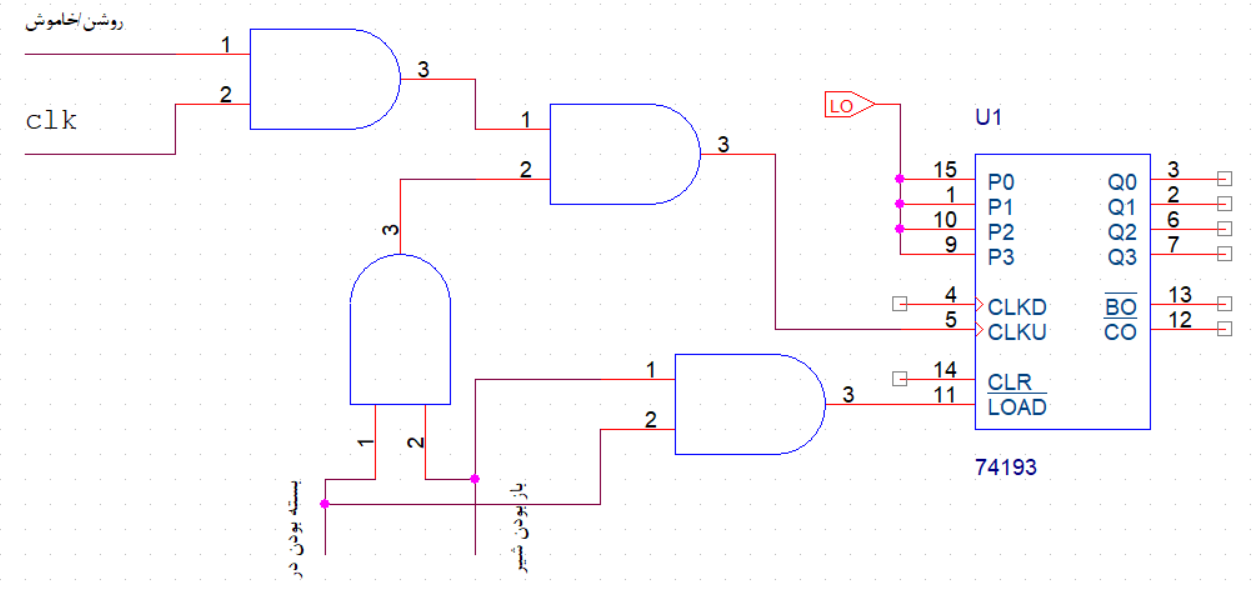
\includegraphics[width=0.8\textwidth]{Circuit1}
\caption{\label{fig:Circuit1}Washing machine timer circuit1.}
\end{figure}

 Now, if conditions are available, our circuit starts to count from 0 to 16, but the things we need are as follows. The outputs are listed in order 1 to 5, respectively

 \begin{table}[H]
\caption{Outputs}
\centering
\begin{tabular}{|*{4}{c|}}
\hline
\multicolumn{2}{|c}{Cold washing} & \multicolumn{2}{|c|}{Hot washing} \\ \hline
0000-0001 & 1 & 0000-0001 & 1 \\
0010-0100 & 3 & 0010-0100 & 2  \\
0101-0110 &4 & 0101-0111 & 3 \\
0111-1000 & 5 &1000-1001 & 4 \\
  &   &1010-1011 & 5 \\
\hline
\end{tabular}
\end{table}

For convenience and to create the above conditions, we connect 4-bit output counts to one another. And we use 2 dicer ones, one for washing with cold water and another for hot water washing. Connect the cold or hot water input signal to enable one dicer and another to connect it to one another so that we can switch between states.

For example, for the number one lamp, as shown in the table. We need  OR to output 0 and 1 dictories of hot water and output 0 and 1 dick in cold water and work the same way for the rest of the outputs. And connect the inputs A through D to the outputs of the previous circuit.
 \begin{figure}[H]
\centering
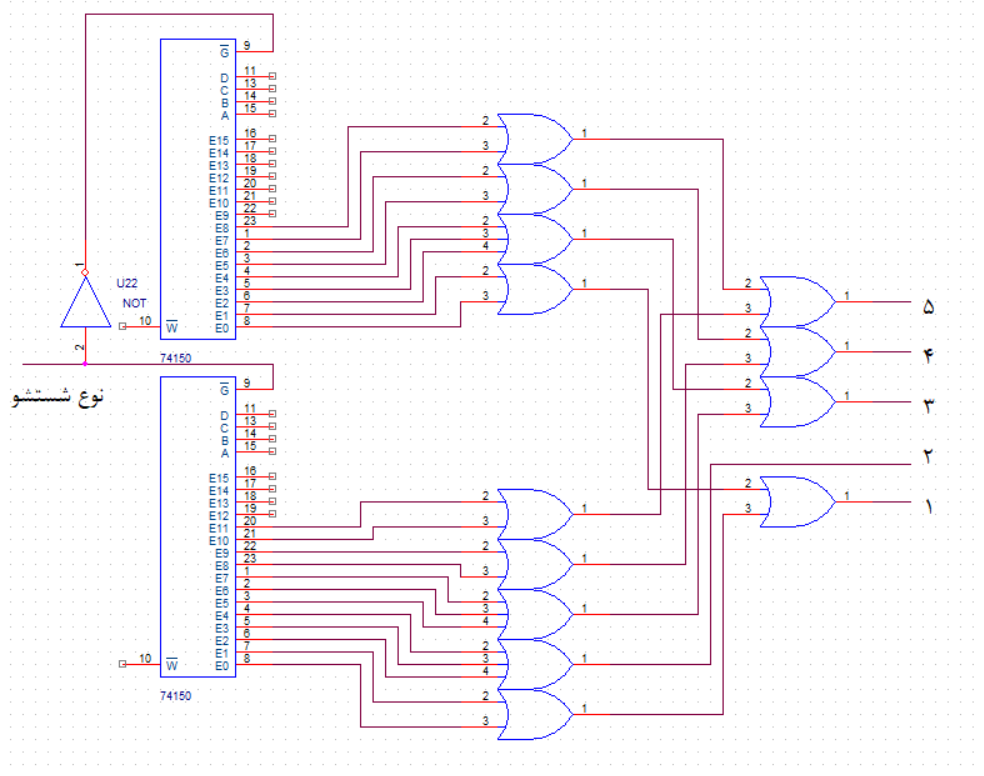
\includegraphics[width=0.8\textwidth]{Circuit2}
\caption{\label{fig:Circuit2}Washing machine timer circuit2.}
\end{figure}

\end{document}